\documentclass{ximera}

\input{../../../preamble.tex}


\definecolor{fvdnavy}{HTML}{071D43}
\definecolor{fvdcyan}{HTML}{20BFC6}
\definecolor{fvdcyanlight}{HTML}{EFFCFB}
\definecolor{fvdmagenta}{HTML}{F10D69}
\definecolor{fvdmagentalight}{HTML}{FFF1F7}
\definecolor{fvdtext}{HTML}{163044}





%=================================================
% Pedagogische omgevingen
% PDF: tcolorbox
% HTML: learning-box
%=================================================

\newenvironment{voorkennis}
{%
    \ifdefined\HCode
        \HCode{%
<section class="learning-box learning-box--prior">
<div class="learning-box__header">
<span class="learning-box__icon" aria-hidden="true"></span>
<span class="learning-box__title">Voorkennis</span>
</div>
<div class="learning-box__content">
        }%
        \begin{itemize}
    \else
       \begin{tcolorbox}[
    enhanced,
    breakable,
    colback=fvdcyanlight,
    colframe=fvdcyan,
    coltext=fvdtext,
    boxrule=0.5pt,
    leftrule=4pt,
    arc=4mm,
    outer arc=4mm,
    left=7mm,
    right=6mm,
    top=5mm,
    bottom=5mm,
    before skip=6mm,
    after skip=6mm,
    title=Voorkennis,
    coltitle=fvdcyan,
    fonttitle=\bfseries\Large,
    attach title to upper={\par\smallskip},
    boxed title style={
        empty,
        left=0mm,
        right=0mm,
        top=0mm,
        bottom=0mm
    },
    overlay={
        \draw[
            fvdcyan,
            line width=0.5pt
        ]
        ([xshift=42mm,yshift=-13mm]frame.north west)
        --
        ([xshift=-7mm,yshift=-13mm]frame.north east);
    }
]
        \begin{itemize}
    \fi
}
{%
    \end{itemize}
    \ifdefined\HCode
        \HCode{%
</div>
</section>
        }%
    \else
        \end{tcolorbox}
    \fi
}


\newenvironment{leerdoelen}
{%
    \ifdefined\HCode
        \HCode{%
<section class="learning-box learning-box--goals">
<div class="learning-box__header">
<span class="learning-box__icon" aria-hidden="true"></span>
<span class="learning-box__title">Leerdoelen</span>
</div>
<div class="learning-box__content">
        }%
        \begin{itemize}
    \else
\begin{tcolorbox}[
    enhanced,
    breakable,
    colback=fvdmagentalight,
    colframe=fvdmagenta,
    coltext=fvdtext,
    boxrule=0.5pt,
    leftrule=4pt,
    arc=4mm,
    outer arc=4mm,
    left=7mm,
    right=6mm,
    top=5mm,
    bottom=5mm,
    before skip=6mm,
    after skip=6mm,
    title=Leerdoelen,
    coltitle=fvdmagenta,
    fonttitle=\bfseries\Large,
    attach title to upper={\par\smallskip},
    boxed title style={
        empty,
        left=0mm,
        right=0mm,
        top=0mm,
        bottom=0mm
    },
    overlay={
        \draw[
            fvdmagenta,
            line width=0.5pt
        ]
        ([xshift=42mm,yshift=-13mm]frame.north west)
        --
        ([xshift=-7mm,yshift=-13mm]frame.north east);
    }
]
        \begin{itemize}
    \fi
}
{%
    \end{itemize}
    \ifdefined\HCode
        \HCode{%
</div>
</section>
        }%
    \else
        \end{tcolorbox}
    \fi
}


\addPrintStyle{../../..}

\title{Oefeningen — Stijgen, dalen en extrema}
\author{Ingmar Herreman}

\begin{document}

% FVD_CHAPTER_DATA_START
% Automatisch gegenereerd uit index.tex.
% Niet handmatig aanpassen.
\fvdchapterdata{5}{Het gedrag van functies beschrijven}{2}
% FVD_CHAPTER_DATA_END




\fvdchapterdata{5}{Het gedrag van functies beschrijven}{2}

\maketitle
\FVDbeginExercises

\begin{opmerking}
De oefeningen met \(\blacklozenge\) zijn essentieel.
Om het leerplandoel op niveau \emph{analyseren} te bereiken moet je niet alleen
verloop kunnen aflezen, maar ook verschillende voorstellingen verbinden,
redeneringen beoordelen en kenmerken interpreteren.
\end{opmerking}

\FVDsection{Basis — verloop correct lezen}

\begin{oefening}[Stijgend, dalend of constant?]{\oefB\ESS}
Een functie \(f\) heeft het volgende verloop:
\[
\begin{array}{c|ccccccc}
x&-5&&-1&&2&&6\\ \hline
f&&\nearrow&4&\searrow&1&\longrightarrow&1
\end{array}
\]

\begin{question}
Op welk interval is \(f\) stijgend?
\begin{oplossing}
Op \([-5,-1]\).
\end{oplossing}
\end{question}

\begin{question}
Op welk interval is \(f\) dalend?
\begin{oplossing}
Op \([-1,2]\).
\end{oplossing}
\end{question}

\begin{question}
Waar is \(f\) constant?
\begin{oplossing}
Op \([2,6]\).
\end{oplossing}
\end{question}
\end{oefening}

\begin{oefening}[Extremumplaats, -waarde en -punt]{\oefB\ESS}
Een functie heeft in \(x=3\) een lokaal maximum met functiewaarde \(7\).

\begin{question}
Geef de extremumplaats, extremumwaarde en het extremumpunt.
\begin{oplossing}
Extremumplaats: \(3\). Extremumwaarde: \(7\).
Extremumpunt: \((3,7)\).
\end{oplossing}
\end{question}
\end{oefening}

\begin{oefening}[Lees de grafiek]{\oefB\ESS}
Beschouw:
\[
f(x)=x^3-3x.
\]

\begin{center}
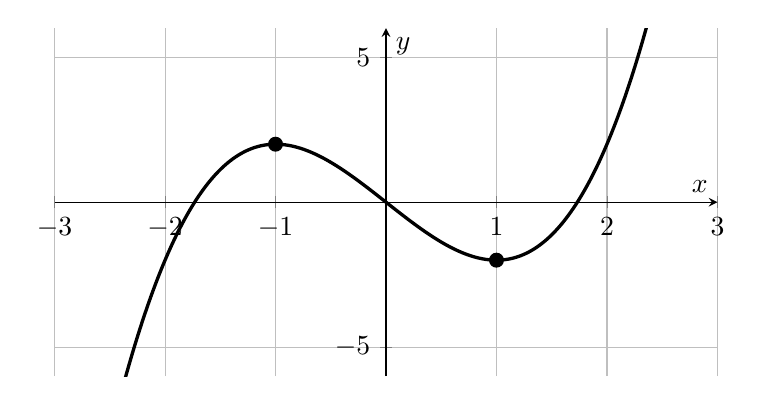
\begin{tikzpicture}
\begin{axis}[
 width=10cm,height=6cm,axis lines=middle,
 xmin=-3,xmax=3,ymin=-6,ymax=6,
 xlabel={$x$},ylabel={$y$},grid=both,samples=200
]
\addplot[very thick,domain=-2.4:2.4] {x^3-3*x};
\addplot[only marks,mark=*,mark size=2.5pt] coordinates {(-1,2) (1,-2)};
\end{axis}
\end{tikzpicture}
\end{center}

\begin{question}
Geef de intervallen waarop \(f\) stijgt en daalt.
\begin{oplossing}
Grafisch:
\[
f\text{ stijgt op }]-\infty,-1]\text{ en }[1,+\infty[
\]
en daalt op
\[
[-1,1].
\]
\end{oplossing}
\end{question}

\begin{question}
Geef de lokale extrema.
\begin{oplossing}
Lokaal maximum: \(f(-1)=2\), met punt \((-1,2)\).
Lokaal minimum: \(f(1)=-2\), met punt \((1,-2)\).
\end{oplossing}
\end{question}
\end{oefening}

\begin{oefening}[Teken en verloop niet verwarren]{\oefB\ESS}
Beoordeel telkens de uitspraak.

\begin{question}
``Als \(f(x)>0\), dan is \(f\) stijgend.''
\begin{oplossing}
Fout. Positief zegt dat de grafiek boven de \(x\)-as ligt; stijgend zegt
dat functiewaarden toenemen wanneer \(x\) toeneemt.
\end{oplossing}
\end{question}

\begin{question}
``Een dalende functie kan positieve functiewaarden hebben.''
\begin{oplossing}
Juist. Bijvoorbeeld \(f(x)=1/x\) op \(]0,+\infty[\).
\end{oplossing}
\end{question}

\begin{question}
``Als een functie van stijgend naar dalend overgaat, ontstaat grafisch een lokaal maximum.''
\begin{oplossing}
Juist.
\end{oplossing}
\end{question}
\end{oefening}

\FVDsection{Verdieping — kenmerken verbinden}

\begin{oefening}[Van verlooptabel naar grafiek]{\oefU\ESS}
Gegeven:
\[
\begin{array}{c|ccccccc}
x&-\infty&&-2&&3&&+\infty\\ \hline
f&&\nearrow&5&\searrow&-1&\nearrow&
\end{array}
\]

\begin{question}
Beschrijf volledig het verloop en de extrema.
\begin{oplossing}
\(f\) stijgt tot \(x=-2\), daalt van \(-2\) tot \(3\) en stijgt daarna.
Er is een lokaal maximum \((-2,5)\) en een lokaal minimum \((3,-1)\).
\end{oplossing}
\end{question}

\begin{question}
Schets een mogelijke grafiek. Is die grafiek uniek?
\begin{oplossing}
Elke schets die door \((-2,5)\) en \((3,-1)\) loopt en het aangegeven
verloop respecteert, is mogelijk. De grafiek is niet uniek: de verlooptabel
legt niet alle functiewaarden vast.
\end{oplossing}
\end{question}
\end{oefening}

\begin{oefening}[Lokaal of globaal?]{\oefU\ESS}
Een functie op \([-5,6]\) heeft lokale maxima
\[
f(-2)=4,\qquad f(4)=7
\]
en lokale minima
\[
f(1)=-3,\qquad f(6)=0.
\]
Verder geldt \(f(-5)=5\).

\begin{question}
Welk gegeven punt levert de grootste functiewaarde?
\begin{oplossing}
\(x=4\), want \(f(4)=7\).
\end{oplossing}
\end{question}

\begin{question}
Leg uit waarom ``lokaal maximum'' niet hetzelfde betekent als ``globaal maximum''.
\begin{oplossing}
Een lokaal maximum wordt alleen met naburige functiewaarden vergeleken.
Een globaal maximum moet groter dan of gelijk zijn aan alle functiewaarden
op het volledige beschouwde domein.
\end{oplossing}
\end{question}
\end{oefening}

\begin{oefening}[Foutenanalyse]{\oefU\ESS}
Een leerling zegt:

``De grafiek ligt tussen \(x=1\) en \(x=4\) boven de \(x\)-as.
De functie is daar dus stijgend.''

Analyseer deze redenering.

\begin{oplossing}
De conclusie volgt niet. Boven de \(x\)-as liggen betekent \(f(x)>0\).
Om te besluiten dat \(f\) stijgt, moeten functiewaarden toenemen wanneer
\(x\) toeneemt. De leerling verwart tekenverloop met stijgen/dalen.
\end{oplossing}
\end{oefening}

\begin{oefening}[Van context naar wiskunde — en terug]{\oefU\ESS}
De hoogte \(h(t)\) van een drone verloopt als volgt:
\[
\begin{array}{c|ccccccccc}
t&0&&3&&5&&8&&12\\ \hline
h&10&\nearrow&55&\longrightarrow&55&\nearrow&70&\searrow&0
\end{array}
\]

\begin{question}
Beschrijf de beweging van de drone in woorden.
\begin{oplossing}
Van \(0\) tot \(3\) s stijgt de drone. Van \(3\) tot \(5\) s blijft hij
op dezelfde hoogte. Van \(5\) tot \(8\) s stijgt hij opnieuw.
Van \(8\) tot \(12\) s daalt hij.
\end{oplossing}
\end{question}

\begin{question}
Wat betekent \(h(8)=70\) in de context?
\begin{oplossing}
Na \(8\) s bevindt de drone zich op \(70\) m hoogte.
\end{oplossing}
\end{question}

\begin{question}
Welke extremumwaarde is uit de tabel globaal maximaal?
\begin{oplossing}
\(70\) m bij \(t=8\) s.
\end{oplossing}
\end{question}
\end{oefening}

\begin{oefening}[Zelf kenmerken combineren]{\oefU\ESS}
Schets een mogelijke functie \(f\) die aan alle voorwaarden voldoet:
\begin{itemize}
  \item \(f\) is stijgend op \(]-\infty,-1]\);
  \item \(f(-1)=3\);
  \item \(f\) is dalend op \([-1,2]\);
  \item \(f(2)=-2\);
  \item \(f\) is stijgend op \([2,+\infty[\);
  \item \(f(0)=0\).
\end{itemize}

\begin{question}
Welke extrema zijn noodzakelijk?
\begin{oplossing}
\((-1,3)\) is een lokaal maximumpunt en \((2,-2)\) een lokaal minimumpunt.
\end{oplossing}
\end{question}

\begin{question}
Is de grafiek uniek bepaald?
\begin{oplossing}
Nee. De voorwaarden bepalen enkele punten en het verloop, maar niet alle
functiewaarden of de exacte vorm tussen de punten.
\end{oplossing}
\end{question}
\end{oefening}

\FVDsection{Gevorderd — redeneren en onderzoeken}

\begin{oefening}[Kan dit?]{\oefG}
Onderzoek of de volgende beschrijving mogelijk is:

\begin{quote}
Een functie is op heel \(\mathbb{R}\) stijgend en heeft in \(x=2\)
een strikt lokaal maximum.
\end{quote}

Motiveer.

\begin{oplossing}
Dit kan niet. Als de functie op heel \(\mathbb{R}\) stijgend is,
dan worden functiewaarden rechts van \(2\) niet kleiner dan \(f(2)\).
Er kan daar dus geen strikt lokaal maximum optreden.
\end{oplossing}
\end{oefening}

\begin{oefening}[Dezelfde extrema, ander verloop]{\oefG}
Construeer twee verschillende grafieken die beide door
\[
(-2,4)\quad\text{en}\quad(3,-1)
\]
gaan, waarbij het eerste punt een lokaal maximum en het tweede een lokaal minimum is.

Zorg ervoor dat de grafieken buiten het interval \([-2,3]\) verschillend gedrag vertonen.
Leg uit welke informatie door de extrema wel en niet vastligt.

\begin{oplossing}
Meerdere antwoorden zijn mogelijk. De extrema leggen lokaal de overgang
stijgend-dalend bij \(-2\) en dalend-stijgend bij \(3\) vast.
Ze bepalen niet de exacte vorm, snelheid van verandering of het globale gedrag
buiten die omgeving.
\end{oplossing}
\end{oefening}

\begin{oefening}[GeoGebra-onderzoek]{\oefG}
Onderzoek in GeoGebra
\[
f_a(x)=x^3-3ax,\qquad a\geq 0.
\]

Gebruik een schuifknop voor \(a\).

\begin{enumerate}
  \item Vergelijk de grafieken voor \(a=0\), \(a=1\), \(a=2\) en \(a=4\).
  \item Beschrijf kwalitatief hoe het aantal en de ligging van de extrema veranderen.
  \item Zoek voor elke gekozen waarde grafisch de intervallen van stijgen en dalen.
  \item Formuleer een vermoeden over wat er gebeurt wanneer \(a\) groter wordt.
  \item Leg uit welke conclusies je rechtstreeks uit de grafiek haalt.
\end{enumerate}

\begin{oplossing}
Voor \(a=0\) is \(f(x)=x^3\) overal stijgend en is er geen lokaal extremum.
Voor positieve \(a\) ontstaat grafisch een lokaal maximum links van de oorsprong
en een lokaal minimum rechts ervan. Naarmate \(a\) groter wordt, liggen die
keerpunten verder uit elkaar. Exacte algebraïsche bepaling met afgeleiden
komt later in de cursus.
\end{oplossing}
\end{oefening}



\end{document}
